\documentclass[12pt,twoside]{third-rep}

\linespread{1.0}
\usepackage{url}
\usepackage{pslatex}
\usepackage[toc,page]{appendix}
\usepackage{longtable}

\usepackage[backend=biber, style=authoryear]{biblatex}
\addbibresource{refs.bib}
\usepackage{csquotes}

\usepackage{listings}
\lstset{
  language=Python,
  numbers=left,
  breaklines=true,
  basicstyle=\ttfamily
}
\lstMakeShortInline[columns=fixed]|

\usepackage{titlesec}
\usepackage{hyperref}
\usepackage{enumitem}
\usepackage{fancyhdr}
\usepackage{subcaption}
\usepackage{threeparttable}

\usepackage{graphicx}
\graphicspath{{img/}}

\pagestyle{fancy}
\fancyhf{}
\fancyhead[LE,RO]{\rightmark}
\fancyhead[RE,LO]{\thepage}
\renewcommand{\headrulewidth}{0pt}

\titleformat{\chapter}[display]
  {\normalfont\bfseries}{}{0pt}{\Large}

\title{Automatic Birdsong Recognition}

\author{Victor F. Lampreia Rodrigues}

\supervisor{Dr. Andrea Schalk}

\reportyear{May 2017}

\abstractfile{tex/abstract.tex}
%\thanksfile{thx.tex}

\begin{document}

\dotitleandabstract

\tableofcontents
%\listoffigures
%\listoftables

\chapter{INTRODUCTION}

The ability to recognise bird species through the sounds they produce has
benefited ornithologists and amateurs in the observation of such creatures in
the wild.
Most birds vocalise, for communicative purposes such as mating, territoral, and
coordination.

Vocalisations are categorised into songs and calls, which differ by the duration
and complexity of the sounds.
Calls are relatively simple in structure and is often breif.
Conversely, songs are usually long sequences of sounds, often featuring
structurally complex and melodic tones.

The trained ear can distinguish birds through their songs and calls, but with
over 10,000 uniquely catalogued species around the world, this becomes a far cry
from practicality.
Some methods have been developed to assist in the identification of species.
The introduction of the use of sonograms for instance has made identification
both faster and more precise for experienced ornithologists, undoubtebly
influincing the breadth and depth of scientific inquiry into the behaviour of
birds.

Current manual and semi-automatic methods for bird sound recognition are limited
by the cost and challenge of analysing enormous amounts of field recordings.
A fully automatic mechanism would be highly advantageous could allow for
large scale, close to real-time or passive classification.

Example applications of such observation technologies include population monitoring
and migration tracking of species in the fields of biogeography and conservation
efforts, as well as the possibility to support public software for the general
birdwatcher.

The problem itself touches on many facets of computer science and engineering,
including digital signal processing and analysis, image recognition,
machine learning, and performance optimization.

\section{Assumptions and Scope}
The primary aim of this project is to research and develop potential methods
for automatic birdsong recognition, which function with little to no user
interaction.
The end-goal is to produce a program which is able to identify the species of
the most prominent bird present in a recording.
It is not the goal of this project to produce commercial software ready for
public consumption.

Recordings used for development and evaluation
originate from arbitrary locations and sources around the world.
They shall not undergo any form of manual selection or processing.
In similar vein, they should also not be subjected to rigorous quality control
aside from what classifications may be provided by sources.
This is to ensure that validation represents real-world performance.\\

For the purposes of this project, some limitations in scope are imposed to
simplify some problem areas:
\begin{itemize}
\item A general level of quality is ensured by selecting only higher quality recordings
      as defined by the data source.
      This is a reasonable restriction which reduces the number of recordings required.
\item The number of species the system should know about is limited to 50
      randomly picked labels.
\item Only bird songs are considered.
      Bird songs differ from calls in complexity, length and context.
      song is usually but not always performed by males.
      a few more details
\end{itemize}


\section{Existing Approaches}
Automatic birdsong recognition has become increasingly popular in the field of
data science the past decade.
Several competitions have taken place to develop
solutions to the problem, each with varying requirements and data.

The MLSP 2013 challenge \parencite{kaggle} for example has lead to a few
successful approaches with a fairly normalised dataset consisting of 645 10
second audio files of 19 individual species, including data which may be used
directly as features for classification.
The most successful entry \parencite{fodor2013} achieved an AUC of 95.6\% using
spectrogram cross-correlation and a binary relavance approach with random forests.

The LifeCLEF 2014 challenge \parencite{lifeclef2014} expanded by offering a much
larger dataset of 14027 non controlled audio files sourced from Xeno-Canto
\parencite{xenocanto}, encompassing 501 different species.
A winning solution \parencite{lasseck2014} achieved an AUC of 91.5\%, with a
precision of 51.1\%.
The solution made use of a combination of audio scene analysis techniques,
spectrogram cross-correlation, and a extremely randomised trees classifier.

The author had also competed in the NIPS 2013 \parencite{nips} competition
using spectrogram segment analysis and spectrogram cross-correlation with an
ensemble of extremely randomised trees classifiers. An AUC of 91.6\% was
achieved.\\

A few commercial software solutions exist, such as Warblr \parencite{warblr} and
Chirpomatic \parencite{chirpomatic} eixst,
although these are typically limited in scope and accuracy.

the previous student

\section{Our Approach}
Our initial approach is inspired by similar sound recognition problems.
Such problems include the recognition of voice, music, animals vocalisations
including whale song, calls, and so on.
It is observed that these problems, while similar in nature, differ in practice.
This is mainly due to the nature of the sound being analysed, as well as
domain knowledge of the structure.

For example, the acoustics of human voice is well studied, and patterns are
easily identified today.
Specialised methods for analysing voice recordings exist, including intonation
etc etc \textbf{add more}.
we have a mapping, we know the words, we dont speak bird noises

Music recognition is trivial in the case of identifying pure reproductions,
the main challenge in this area being noise reduction and distortion compensation.
Music can be easily identified using statistical methods to compare pitch
variations along the duration of the recording.
Bird song however contains many variations and transpositions within the same
species which make it difficult to find an archetypal sequence of pitch
variations.\\

Some approaches to these problems are essentially spectrographic image recognition
tasks, where elements common to specific labels are searched for within a target
example spectrogram.
The simplicity and success of such solutions has driven the direction of this
project.

Our approach uses a combination of computer vision and machine learning
techniques to construct a fully automatic recognition system.
Standard image processing methods are used to process spectrograms and extract
sections of song which may be used to identify a particular species, much like
how an orthonologist visually inspects the song spectra.
These sections are then matched against new samples to be classified through a
multi-class machine learning algorithm.

move bulk of subsections to appendices

\subsection{Process Overview}
The project is divided into four descrete parts.
These follow the logical flow of data:
\begin{enumerate}
  \item \textbf{Collection:}
    Data is sourced from field recordings done in uncontrolled environments.
    The variety provides a good estimate of real-world performance and
    introduces many quality related issues.

  \item \textbf{Preparation and selection:}
    Recordings are filtered and selected to maintain reasonable quality levels.
    Spectrograms are then derived from the recordings.
    This is now the representation that is used throughout the program until
    the feature vector is constructed.

  \item \textbf{Preprocessing and feature extraction:}
    Noise is reduced as much as possible to identify key regions of interest
    within the spectrogram image.
    These are extracted as templates and cross-correlated against other
    recording spectrograms to form a feature vector.

  \item \textbf{Classification and evaluation:}
    The resulting data is then fed to a classifier and evaluated using techniques
    designed to reduce statistical bias.
\end{enumerate}

Each of these procedures are described in detail in their respective sections.
A few of these sections discuss possible alternatives or improvements to the
developed mechanisms.

A regular focus of the project is performance statistics, which is done for each
stage of the program to some granularity.
A report on this is available in appendix xyz.

\subsection{Architecture Overview}
\textbf{diagram of key sections}

Due to the experimental nature of the project, a rigorous architecture has not
been designed ahead of time.
The codebase evolved through several iterations 


\subsection{Implementation Technologies}
All code is written in Python 2.7.
Libraries used include:
\begin{itemize}
  \item open-CV 2.0
\end{itemize}


\chapter{WORKING DATA}

This project bases all mechanisms on one single birdsong representation, the
source field recordings.
This section describes the data used, how it is collected, and prepared for
usage within the program.


\section{Data Source: Xeno-Canto}

Xeno-Canto provides a substantial number of user uploaded field recordings
of various bird species, both calls and songs (\textcite{xenocanto}).
Recordings may originate from any part of the world, may vary extremely in
terms of quality, and any number of species may be present in a single
recording.

Recordings are of varying duration, ranging from 1 to 20 minutes each.
The content may be densely packed, with multiple birds singing simultaneously,
or sparse with long durations of silence.

Xeno-canto provides all audio as dynamic MP3.
These are normalised as described in Section~\ref{sec:prep}

\subsection{Metadata}
Xeno-canto provides the following metadata with each recording:
\begin{itemize}[noitemsep]
  \item Date and time
  \item Recording location
  \item Species recorded
  \item Existence of other species
\end{itemize}

This program only makes use of the prominent species tagged in the recording.
Although not used in our implementation, the location of the recording could be
used to improve the accuracy of the classifier, as some species are restricted
to certain parts of the world.
Including this information in the feature set is very likely to provide a
good accuracy by itself, but without much precision.
It can be used however to narrow down the set of possible species, so long as
special care is taken to account for migration patterns.


\subsection{Automatic Sample Retrieval}
Manually selecting and downloading recordings is a time-consuming process.
A public API does not exist for Xeno-canto, therefore we developed a web scraper
specifically for automatic retrieval.

The scraper allows the user to filter samples on species and on recording quality
before downloading a sample by examining the metadata present in the HMTL.
Filtering may be done by exclusion or selection.

When repeated fetching is required, an interval may be set in order to reduce
strain on Xeno-canto's servers.
Once the interval has been set, the scraper will continuously download samples
at the specified rate until it has been interrupted by the user.\\

The webscraper is written in Python 2.7 using the |lxml| package.

\section{Preparation}\label{sec:prep}
\subsection{Resampling}
Recordings are resampled to 22000 khz to reduce the memory footprint and
processing power required to operate on each recording.
Resampling to 22050 khz was found to have no significant reduction in quality
or information retained, despite the high frequency vocalizations in birdsong.

The right channel of any stereo recordings is discarded.

The source MP3 files are converted into 22kHz 16-bit WAV files.

Resampling and conversion is done using ffmpeg and automated through a shell
script.


\subsection{Spectrogram Construction}
All recordings are processed into spectrograms through a fast fourier transform
(FFTS) method provided by the xxx python library.
This representation provides a visualization of energy present in each frequency
band in function of time.
Each frequency is quantized into discrete bands according to the parameters set.
Time is quantized into etc.
The absolute energy is preserved, we don't lose any information, we gain it.
\textbf{show spectrogram image under waveform of same section}

The following parameters are used:
\begin{itemize}
  \item NFFT: 512
  \item window: Hamming window of 512
  \item n overlap: 75\%
\end{itemize}

See Appendix for details on FFTS.

Frequencies above 10000Hz and below 100Hz are removed from the spectrograms as these do
not contain signals belonging to any bird species \textbf{(cite)}.

\section{Sample Selection}\label{sec:sample_select}
A local database of birdsong samples has been created, using collections
extracted from Xeno-Canto through the described automatic procedure.
Over the course of several days, 2211 total distinct samples have been downloaded
and processed.
189 individual species have been catalogued, with approximately half of these
including more than 10 individual samples.
The top 10 species, and their sample counts are shown in Table~\ref{tab:top10}.
See Appendix~\ref{app:samples} for a full list.
The average length of each recording is approximately 1 minute.

Due to resource limitations imposed by template matching, not all samples
are used in the final evaluation of the algorithm.
Although all samples are processed as described in Section~\ref{sec:prep} and
\ref{sec:preproc}, only a selection is passed through feature extraction and
classification stages.

The following criteria has been found to result in a good balance between
data volume and time cost:
\begin{itemize}
  \item Reject species with less than 20 samples
  \item Retain first 20 samples of each species
  \item Reject species with less than 2000 templates
  \item Keep first 3000 templates of each species
\end{itemize}

To reduce bias samples and templates may instaed be picked at random, however
we did not have time to implement a method for tracking the random sampling.

\begin{table}[!htb]
  \caption{Top 10 species by sample count}\label{tab:top10}
  \centering
    \begin{tabular}{r l}
      Samples & Species Label \\ \hline
      102 & Eurasian Blackcap\\
      101 & Common Blackbird\\
      98  & Eurasian Wren\\
      69  & Common Chiffchaff\\
      66  & Grey-breasted Wood Wren\\
      55  & Spotted Towhee\\
      49  & Garden Warbler\\
      46  & Common Whitethroat\\
      45  & Eurasian Blue Tit\\
      41  & River Warbler\\
    \end{tabular}
\end{table}

The |repository| class facilitates sample rejection and selection based on
several criteria, including class and template counts.

% audio samples (wav): 2211
%  102  Eurasian Blackcap       
%  101  Common Blackbird        
%   98  Eurasian Wren           
%   69  Common Chiffchaff       
%   66  Grey-breasted Wood Wren 
%   55  Spotted Towhee          
%   49  Garden Warbler          
%   46  Common Whitethroat      
%   45  Eurasian Blue Tit       
%   41  River Warbler           
%   40  Great Reed Warbler      
%   39  Rufous-browed Peppershri
%   38  Eurasian Reed Warbler   
%   38  White-breasted Wood Wren
%   38  Yellowhammer            
%   36  Common Grasshopper Warbl
%   35  Northern Mockingbird    
%   32  Common Reed Bunting     
%   32  Corn Bunting            
%   29  Common Cuckoo           
%   28  Common Redstart         
%   27  Common Rosefinch        
%   24  Chestnut-breasted Wren  
%   24  Ortolan Bunting         
%   23  Western Meadowlark      
%   23  Pale-breasted Spinetail 
%   21  European Greenfinch     
%   21  White-throated Toucan   
%   20  Pin-striped Tit-Babbler 
%   19  American Robin          
%   18  Ferruginous Pygmy Owl   
%   16  Barred Antshrike        
%   16  Green-winged Saltator   
%   15  Black-faced Antbird     
%   15  Black-striped Sparrow   
%   15  Lesser Shortwing        
%   14  Plumbeous Vireo         
%   14  Pale-breasted Thrush    
%   14  Plain-tailed Wren       
%   14  Rufous-capped Warbler   
%   14  Swainson's Thrush       
%   14  Channel-billed Toucan   
%   13  White-breasted Tapaculo 
%   13  Common Potoo            
%   13  Tawny Owl               
%   13  Grace's Warbler         
%   13  Greenish Warbler        
%   12  Loggerhead Shrike       
%   11  Great-tailed Grackle    
%   11  Japanese Bush Warbler   
%   11  White-throated Sparrow  
%   11  Collared Owlet          
%   11  Giant Antshrike         
%   11  Undulated Tinamou       
%   10  Rattling Cisticola      
%   10  Painted Bunting         
%   10  Eastern Meadowlark      
%   10  Bell's Vireo            
%   10  Scrub Greenlet          
%   10  Olive Warbler           
%   10  Laughing Falcon         
%    9  Red-winged Blackbird    
%    9  Common Hawk-Cuckoo      
%    9  Yellow-browed Sparrow   
%    9  Slaty-breasted Wood Rail
%    9  Sumichrast's Wren       
%    9  Plain-crowned Spinetail 
%    9  Yellow-eyed Junco       
%    9  Spotted Nightingale-Thru
%    9  Japanese White-eye      
%    8  Southern Yellowthroat   
%    8  Great Tinamou           
%    8  Sooty Antbird           
%    8  Styan's Grasshopper Warb
%    7  Yellow-throated Vireo   
%    7  Connecticut Warbler     
%    7  Hooded Siskin           
%    7  Fire-tufted Barbet      
%    7  Duida Woodcreeper       
%    7  Gartered Trogon         
%    7  Eurasian Treecreeper    
%    7  Buff-browed Foliage-glea
%    7  Eurasian Golden Oriole  
%    7  White-bellied Antpitta  
%    7  Grey Antwren            
%    7  Southern Boubou         
%    6  Recurve-billed Bushbird 
%    6  Golden-crowned Sparrow  
%    6  Splendid Sunbird        
%    6  Moustached Wren         
%    6  Collared Antshrike      
%    6  Violaceous Euphonia     
%    6  Bay Wren                
%    6  Siberian Blue Robin     
%    6  Zigzag Heron            
%    6  Henna-hooded Foliage-gle
%    6  Baillon's Crake         
%    6  Paradise Jacamar        
%    6  Rufous-vented Tapaculo  
%    6  Ashy-headed Greenlet    
%    6  Western Orphean Warbler 
%    6  Spotless Starling       
%    6  Eastern Woodhaunter     
%    6  White-throated Screech O
%    6  Lineated Foliage-gleaner
%    5  Yellow Grosbeak         
%    5  Tanager Finch           
%    5  Foothill Schiffornis    
%    5  Singing Quail           
%    5  Orange-breasted Bushshri
%    5  Esmeraldas Antbird      
%    5  Spectacled Owl          
%    5  Fan-tailed Cuckoo       
%    5  Dark-capped Bulbul      
%    5  Marico Sunbird          
%    5  Yellow-bellied Elaenia  
%    5  Buff-cheeked Greenlet   
%    5  Audubon's Oriole        
%    5  Curve-billed Scythebill 
%    4  White-throated Toucanet 
%    4  Red-fan Parrot          
%    4  California Quail        
%    4  Rufous-tailed Hummingbir
%    4  Black-cowled Saltator   
%    4  Western Wood Pewee      
%    4  Variegated Antpitta     
%    4  Wedge-billed Woodcreeper
%    4  Greater Thornbird       
%    4  Blue-chested Hummingbird
%    4  Green-backed Sparrow    
%    4  Varied Bunting          
%    4  Long-billed Pipit       
%    4  Ferruginous Partridge   
%    4  White-vented Violetear  
%    4  Wedge-tailed Grass Finch
%    3  White-shouldered Antbird
%    3  Blue-winged Pitta       
%    3  White-spectacled Warbler
%    3  Jerdon's Leafbird       
%    3  Olive Thrush            
%    3  Azure Jay               
%    3  Johannes's Tody-Tyrant  
%    3  Short-billed Leaftosser 
%    3  Japanese Quail          
%    3  Chestnut-bellied Thrush 
%    3  Crested Lark            
%    3  Emerald Toucanet        
%    3  Greater Hoopoe-Lark     
%    3  Golden-rumped Euphonia  
%    3  Chestnut-bellied Nuthatc
%    3  Forest Elaenia          
%    3  Moustached Puffbird     
%    3  Choco Tapaculo          
%    3  White-fronted Honeyeater
%    3  White-necked Puffbird   
%    2  Bahama Oriole           
%    2  Arafura Fantail         
%    2  Yellow-crowned Elaenia  
%    2  Plush-crested Jay       
%    2  Scarlet-rumped Trogon   
%    2  Bronzy Jacamar          
%    2  Grey-throated Warbler   
%    2  Pearly Antshrike        
%    2  White-eared Brown Dove  
%    2  Philippine Coucal       
%    2  Flammulated Bamboo Tyran
%    2  Russet Nightingale-Thrus
%    2  Little Cuckoo-Dove      
%    2  White-naped Jay         
%    2  Hepatic Tanager         
%    2  Pririt Batis            
%    2  Solitary Tinamou        
%    2  Black-goggled Tanager   
%    2  Jerdon's Nightjar       
%    2  Cuban Vireo             
%    1  Yellow-breasted Boatbill
%    1  Cherrie's Antwren       
%    1  Sand Martin             
%    1  Negros Scops Owl        
%    1  Yellow-breasted Pipit   
%    1  Curve-winged Sabrewing  
%    1  Streak-breasted Treehunt
%    1  Sombre Rock Chat        
%    1  Mountain Wren-Babbler   
%    1  Eastern Nicator         
%    1  Emei Shan Liocichla     
%    1  Tiny Tyrant-Manakin     
%    1  Crimson-backed Tanager  
%    1  Green-chinned Euphonia  
%    1  Winifred's Warbler      


\chapter{FEATURE EXTRACTION}

\section{Template Extraction}


\section{Template Matching}

\section{Useful Feature Identification}

Orthonologists use this and that.
We're taking an image recognition based approach

show spectrograms of various species to show differences

Variations in amplitude along the song are not taken into account but may be a 
useful feature to consider.

Direct spectral information such as mean energy per frequency bin is not taken
although this can be a useful statistic to help identify the species.


%\subsection{Spectrogram Preprocessing}\label{sec:preproc}

Before any features can be extracted, their pixel boundaries must be found.
This is a non-trivial problem due to noise and recording artefacts
that may be present in each spectrogram.
The complexity of the problem is risen by the inconsistency of these from sample
to sample.

Figure~\ref{fig:sgram_noise} shows an example of a noisy spectrogram.
Notice how background noise makes it difficult to find the exact boundary of
some of the vocalisations.
\textbf{define noise, both background and unwanted signal also rewrite the notice}

\begin{figure}[h]
  \centering

  \caption{Considerably noisy spectrogram of a segment of xbird song.}
  \label{fig:sgram_noise}
\end{figure}

Even after quality prefiltering done when downloading recordings from
Xeno-canto, noise levels remain at undesireable levels.

Removing noise and unwanted artefacts manually is precise, although tedious.
Because a high number of samples is required for our approach, we developed an
automatic noise reduction stage, as doing so manually would be far too
impractical at this scale.
Standard computer vision techinques for noise reduction were used, as well as
techniques for discrete object identification.

\subsubsection{The mechanism}
A filter is first applied to the spectrogram, which reduces the noise in the
image by smoothing just enough until granular noise is reduced sufficiently
(Figure~\ref{fig:preproc_vis_filter}).
This is accomplished using a Gaussian filter with a 5x5 kernel and sigma of 0.
\textbf{sigma 0??}
Median filtering was also tested. \textbf{so what happened?}

The image is then thresholded using a thresholding algorithm
(Figure~\ref{fig:preproc_vis_thresh}).
Otsu's binarization thresholding technique was used to select an optimal
threshold value.
Because of pixel intensity inconsistencies throughout individual spectrograms,
specifically in areas where noise is prominent, an adaptive thresholding
algorithm was also tested.
This did not appear to provide generally better results.

Further noise reduction is then performed using dilation and erosion
(Figure~\ref{fig:preproc_vis_dilation1}),
which removes small segments and joins pixel groups which are in close proximity
to each other.
Notice that the order of operations is flipped here since we are working with
an inverted spectrogram.
Dilation and erosion is then performed a second time for larger segments
(Figure~\ref{fig:preproc_vis_dilation2}),
A kernel size of 3x3 and 7x7 were used for small and large segments, respectively.

Most remaining holes are then filled using a closing morphology algorithm,
using an ellipse of size 3x3 (Figure~\ref{fig:preproc_vis_closing}).

\begin{figure}[h]
  \centering
  \begin{subfigure}[b]{0.55\textwidth}

    \caption{Gaussian filter, $k=5x5, \sigma=0$}
    \label{fig:preproc_vis_filter}
  \end{subfigure}
  \begin{subfigure}[b]{0.55\textwidth}

    \caption{Otsu's threshold}
    \label{fig:preproc_vis_thresh}
  \end{subfigure}
  \begin{subfigure}[b]{0.55\textwidth}

    \caption{Dilation followed by erosion, $k=3x3$}
    \label{fig:preproc_vis_dilation1}
  \end{subfigure}
  \begin{subfigure}[b]{0.55\textwidth}

    \caption{Dilation followed by erosion, $k=7x7$}
    \label{fig:preproc_vis_dilation2}
  \end{subfigure}
  \begin{subfigure}[b]{0.55\textwidth}

    \caption{Closing, 3x3 ellipse}
    \label{fig:preproc_vis_closing}
  \end{subfigure}
  \caption{Preprocessing stages in order.}
  \label{fig:preproc_vis}
\end{figure}

Following these procedures the spectrogram is transformed into a binary image
consisting of discrete pixel segments.
This representation simplifies the extraction procedure as described in
Section~\ref{sec:extract}.


\subsubsection{Granularity considerations}\label{sec:granularity}
It is important to consider and evaluate the granularity to aim for when
isolating sections of song.
It is not clear if large sections of song would perform better than smaller,
individual vocalisations.
An evaluation should therefore be performed to determine the best granularity.

Trialing different granularities bears the weight of template matching for all
new templates, which is extremely time consuming.

Further, achieving consistent granularity across all spectrograms is not a trivial
task, and is certainly not possible if a single parameter set is used for
all spectrograms.

A loose aim is therefore taken to extract the smallest possible non-singular
vocalisations.
This of course does not always work, but the developed mechanism gives good
results.

\subsubsection{Quality and consistency}
It is difficult to arrive at a single set of optimal parameters that work
well across all spectrograms.
An adaptive method is therefore suggested (but not implemented):
Preprocessing parameters may be specified on a per-recording basis if prior
knowledge is gathered for expected vocalisation/section counts, template
dimensions, and frequency range.
Since there is no known structured source of data for this, it is necessary to
manually specify these on a per-species basis.
Alternatively a fully automatic method is conceivable by feeding back the
classification results with each granularity setting.
This however would be incredibly time consuming on standard hardware, and may
be sensitive to other factors in the classification pipeline.

Consistent quality becomes less of a concern as the number of samples used for
training increases.
It can be shown that as the sample count increases, the number of valid templates
tends to increase.
The number of noise also increases, however these do not intercorrelate as valid
templates do, and are handled well by less sensitive classifiers such as
random forests (\textcite{marko2004}).

Quality is therefore moderated after preprocessing in the selection stage as
described in Section~\ref{sec:template_select}.

\section{Template Extraction}
Before we can extract template images for cross-correlation, they must first be
identified in the source spectrograms.
For this to be viable at any level of consistency, spectrograms must undergo
noise reduction and segmentation.
This section details the mechanisms developed for preprocessing spectrogram
images and filtering segments so that only relevant templates are included for
extraction.

Each spectrogram is processed in sequence using functionality provided by the
Python OpenCV library, and immediately stored on disk.
Parallelisation is possible here, but the computational cost of this stage is
not large enough to justify sparing development time on this aspect at the time.

\subsection{Spectrogram Preprocessing}\label{sec:preproc}

Before any features can be extracted, their pixel boundaries must be found.
This is a non-trivial problem due to noise and recording artefacts
that may be present in each spectrogram.
The complexity of the problem is risen by the inconsistency of these from sample
to sample.

Figure~\ref{fig:sgram_noise} shows an example of a noisy spectrogram.
Notice how background noise makes it difficult to find the exact boundary of
some of the vocalisations.
\textbf{define noise, both background and unwanted signal also rewrite the notice}

\begin{figure}[h]
  \centering

  \caption{Considerably noisy spectrogram of a segment of xbird song.}
  \label{fig:sgram_noise}
\end{figure}

Even after quality prefiltering done when downloading recordings from
Xeno-canto, noise levels remain at undesireable levels.

Removing noise and unwanted artefacts manually is precise, although tedious.
Because a high number of samples is required for our approach, we developed an
automatic noise reduction stage, as doing so manually would be far too
impractical at this scale.
Standard computer vision techinques for noise reduction were used, as well as
techniques for discrete object identification.

\subsubsection{The mechanism}
A filter is first applied to the spectrogram, which reduces the noise in the
image by smoothing just enough until granular noise is reduced sufficiently
(Figure~\ref{fig:preproc_vis_filter}).
This is accomplished using a Gaussian filter with a 5x5 kernel and sigma of 0.
\textbf{sigma 0??}
Median filtering was also tested. \textbf{so what happened?}

The image is then thresholded using a thresholding algorithm
(Figure~\ref{fig:preproc_vis_thresh}).
Otsu's binarization thresholding technique was used to select an optimal
threshold value.
Because of pixel intensity inconsistencies throughout individual spectrograms,
specifically in areas where noise is prominent, an adaptive thresholding
algorithm was also tested.
This did not appear to provide generally better results.

Further noise reduction is then performed using dilation and erosion
(Figure~\ref{fig:preproc_vis_dilation1}),
which removes small segments and joins pixel groups which are in close proximity
to each other.
Notice that the order of operations is flipped here since we are working with
an inverted spectrogram.
Dilation and erosion is then performed a second time for larger segments
(Figure~\ref{fig:preproc_vis_dilation2}),
A kernel size of 3x3 and 7x7 were used for small and large segments, respectively.

Most remaining holes are then filled using a closing morphology algorithm,
using an ellipse of size 3x3 (Figure~\ref{fig:preproc_vis_closing}).

\begin{figure}[h]
  \centering
  \begin{subfigure}[b]{0.55\textwidth}

    \caption{Gaussian filter, $k=5x5, \sigma=0$}
    \label{fig:preproc_vis_filter}
  \end{subfigure}
  \begin{subfigure}[b]{0.55\textwidth}

    \caption{Otsu's threshold}
    \label{fig:preproc_vis_thresh}
  \end{subfigure}
  \begin{subfigure}[b]{0.55\textwidth}

    \caption{Dilation followed by erosion, $k=3x3$}
    \label{fig:preproc_vis_dilation1}
  \end{subfigure}
  \begin{subfigure}[b]{0.55\textwidth}

    \caption{Dilation followed by erosion, $k=7x7$}
    \label{fig:preproc_vis_dilation2}
  \end{subfigure}
  \begin{subfigure}[b]{0.55\textwidth}

    \caption{Closing, 3x3 ellipse}
    \label{fig:preproc_vis_closing}
  \end{subfigure}
  \caption{Preprocessing stages in order.}
  \label{fig:preproc_vis}
\end{figure}

Following these procedures the spectrogram is transformed into a binary image
consisting of discrete pixel segments.
This representation simplifies the extraction procedure as described in
Section~\ref{sec:extract}.


\subsubsection{Granularity considerations}\label{sec:granularity}
It is important to consider and evaluate the granularity to aim for when
isolating sections of song.
It is not clear if large sections of song would perform better than smaller,
individual vocalisations.
An evaluation should therefore be performed to determine the best granularity.

Trialing different granularities bears the weight of template matching for all
new templates, which is extremely time consuming.

Further, achieving consistent granularity across all spectrograms is not a trivial
task, and is certainly not possible if a single parameter set is used for
all spectrograms.

A loose aim is therefore taken to extract the smallest possible non-singular
vocalisations.
This of course does not always work, but the developed mechanism gives good
results.

\subsubsection{Quality and consistency}
It is difficult to arrive at a single set of optimal parameters that work
well across all spectrograms.
An adaptive method is therefore suggested (but not implemented):
Preprocessing parameters may be specified on a per-recording basis if prior
knowledge is gathered for expected vocalisation/section counts, template
dimensions, and frequency range.
Since there is no known structured source of data for this, it is necessary to
manually specify these on a per-species basis.
Alternatively a fully automatic method is conceivable by feeding back the
classification results with each granularity setting.
This however would be incredibly time consuming on standard hardware, and may
be sensitive to other factors in the classification pipeline.

Consistent quality becomes less of a concern as the number of samples used for
training increases.
It can be shown that as the sample count increases, the number of valid templates
tends to increase.
The number of noise also increases, however these do not intercorrelate as valid
templates do, and are handled well by less sensitive classifiers such as
random forests (\textcite{marko2004}).

Quality is therefore moderated after preprocessing in the selection stage as
described in Section~\ref{sec:template_select}.


\subsection{Basic Selection and Extraction}\label{sec:template_select}
With optimal results the segments represent parts of song at the desired
granularity, from elements to phrases.
This is unfortunately not the case.
Noise may persist after preprocessing, and new deformations may appear, such as
incorrectly joined or incomplete segments.

Some effort is taken to reduce the number of undesireable templates.
In addition to noise, undesireable templates include extremely specific or
extremely generalised templates.

For example, if a sound is featured in a single instance of bird song, but not
in any other recording of songs of that species, then it is an extreme outlier,
which may occur due to a bird's individual expression or external sources.
It is non trivial to detect outliers during feature extraction, but because
random forests are generally insensitive to this type of outlier, we do not
treat these in this stage.

On the other hand, generalised templates are easier to detect.
Such templates will have a very faint structure (low contrast), or a complete
lack of structure.
These may be analysed directly and ignored, as they are likely to correlate,
although very weakly, to the majority of spectrograms irrespective of the
species.

Although these rejections bring a theoretical boost to classifier accuracy and
performance, they mainly benefit performance by reducing the number of
cross-correlations computed.

\subsubsection{Selection mechanism}
Complete elimination of all undesireable features is impossible without also
removing desireable features.
A balance must therefore be struck, in both preprocessing and selection stages.
Performing selection manually is extremely time consuming given the quantity
of pixel sections.
Selection is therefore done automatically by considering the dimensionality and
pixel values of each template.\\


Templates with the following properties are automatically rejected:
\begin{itemize}[noitemsep]
  \item \textbf{Area smaller than 50 pixels:} Templates with small dimensions
    are too small to be of any significance and are most likely noise or
    artefacts from preprocessing;

  \item \textbf{Area larger than 10000 pixels:} Templates with extremely large
    dimensions are most likely artefacts from preprocessing, high intensity
    noise or continuous external noises.
    It is possible for sections of song to be merged together into a single
    pixel region due to preprocessing errors.

  \item \textbf{Minimum pixel intensity greater than the average for the
    spectrogram:} attempt at reducing "boring" templates
    but it doesnt make sense
\end{itemize}


\subsubsection{Extraction mechanism}\label{sec:extract}

A bounding box is computed for the contours of each segment, which is then used
to extract a template from the original spectrogram image.
Once selection is performed for a particular pixel region, it's bounding box is
expanded by 10 pixels in each direction, and that region is extracted from the
original, unprocessed spectrogram.
This forms a single template.
The template is then blurred using Gaussian filtering with a sigma of 1.5.

The reason for blurring is to reduce the dimensionality of the template, which
brings performance boosts to template matching (described in
Section~\ref{sec:ccm}) since the template may now be reduced in size.

Blurring the template also improves it's generality, which makes matches more
likely.
Special consideration must be taken in order to ensure templates are not overly
generalised, as this will cause excess ambiguity amongst templates.



\subsection{Guided Template Elimination}
It is desireable to reduce the template count further by recognizing aspects which
make for good templates. This subsection outlines some speculative options for
selecting better templates, and reducing those which would have a low importance
score after training and classification.

\subsubsection{Image contrast}
It can be argued that templates with low local contrast contain insufficient
information to be meaningful in any way during template matching.
Templates with a low contrast match against much of any image, resulting in an
increase in noise.
Implicitly \textbf{is implicitly the right word?} such templates have a high
correlation with not only the species from which it was extracted but with all
species.
\textbf{show some images, maybe graphs of correlation}

\subsubsection{Spatial inclusion}
Due to the imperfect nature of the preprocessing methods used, gaps and
inconsistencies in structure appear in the thresholded spectrogram.
These inconsistencies are present also in repeated components in a bird song,
at all levels of granularity.
This causes multiple templates to be extracted for a single component in some
instances, and single larger blocks to be extracted in others.

In many of these cases, one template's bounding box intersects or is contained
entirely within another template's bounding box.
Merging these templates by extracting the bounding box of the union of the two
or more templates may result in more consistent extractions.
\textbf{show some images}

Similarly, templates which are sufficiently close to eachother may be merged,
but care must be taken not to form extremely large templates.

\subsubsection{Variation in granularity}
There exists a variance in granularity for the extracted templates, in which
some sections of song are mostly connected to form a single template, and others
are disconnected, leaving templates with single syllables \textbf{right word?}
and templates with entire sections of song.
This is a similar to the observation in \textbf{spatial inclusion}.

\textbf{what to do about it}
\textbf{is it a problem}


\subsubsection{inter-template correlation}
some templates may correlate with eachother, should they be merged?

It can also be argued that templates with little to know intercorrelation may be
independent anomalies such as noise in the signal or other sounds irrelevant to
the subject species.

\subsubsection{Species-specific template statistics}
It may be possible to use information regarding average dimensionality and mean
frequency information to determine the relevance likelyhood of a particular template.
Such metrics require an existing set of validated templates, which may be gathered
by filtering a non discriminated set of templates by their measures importances.

\section{Feature Engineering}\label{sec:ccm}
With a collection of extracted templates from each spectrogram, feature vectors
can be constructed to distinguish between various bird species.
This is done through cross-correlation mapping, an image recognition algorithm.
A feature vector is derived from the results of cross-correlating all
templates against samples of known species.
These feature vectors are then used to train a machine learning algorithm to
classify new recordings from their spectrograms.

This section describes the mechanisms used to perform cross-correlation mapping
for feature vector construction and a short analysis of the computational
expense involved.

\subsection{Batch Processing}
Once initial reductions have been made through the selection process,
further processing is batched in groups of four species, which are selected in
random order without replacement.
Each batch undergoes template matching, the results of which are stored on disk.
Once a batch is completed it is merged with previous results by cross-template
matching the new templates against the old spectrograms and the old templates
against the new spectrograms.
The new results are appended to the old feature vectors and stored on disk.

This is an effective method for dividing work into managable chunks while storing
intermediate results.
The cost analysis in the following section justifies the need for batching.

\subsection{Template Matching}
Template matching is a method for computing the similarity of an image within
another.
We use a normalised cross-correlation method for template matching.
This mode was chosen over squared-difference and cosine-coefficient because it
has been used with good results in similar spectrogram template matching tasks
(\textcite{lasseck2013}).
Normalisation is used to reduce the effect of background noise in the
spectrogram images.

The result of cross-correlation is a 2-dimensional vector of equal dimensions to
the target image, where values are normalised from 0 to 1 (Figure~\ref{fig:ccm}).
Greater values indicate a higher level of correlation for the template in that
area.
This can be thought of and visualised as a heatmap of the template's correlation.

\begin{figure}[t!]
  \centering
  \begin{subfigure}[t]{0.5\textwidth}
    \centering
    \caption{}
  \end{subfigure}
  \begin{subfigure}[t]{0.5\textwidth}
    \centering
    \caption{}
  \end{subfigure}
  \begin{subfigure}[t]{0.5\textwidth}
    \centering
    \caption{}
  \end{subfigure}
  \caption{Visualisation of a cross-correlation mapping (c) of template (a) against
  spectrogram (b)}
  \label{fig:ccm}
\end{figure}

Section~\ref{sec:feature_imp} discusses the mechanism for and analysis of feature
importance.

\subsubsection{Implementation and cost}
We use Open-CV's |matchTemplate| function with the normalised CCM method.
It's implementation uses a Fourer analysis approach for improved performance over
the traditional raw statistical methods.
This works by first applying a FFT to the template and target image before
performing the cross-correlation.
\textbf{cant find ref, look at code?}

Even with such optimizations, template matching takes a considerable amount of
time.
Template matching takes on average x minutes per template, given
mean size of m and n pixels for spectrograms and templates respectively.
Considering the quantity of templates being analysed, the time required quickly
amounts to days.

To gain insight into how the requirements respond to the size of a
spectrogram, a feature extraction run was performed for 80 spectrograms of
varying sizes, with 12204 templates.
Spectrograms and templates were selected at random following the same selection
and filtering procedures described in previous sections.
Total time to completion was approximately 22 hours on the machine listed in
Appendix~\ref{app:machine}.\\

\begin{figure}[!htb]
  \centering
  \begin{subfigure}[b]{0.5\textwidth}
    \centering
    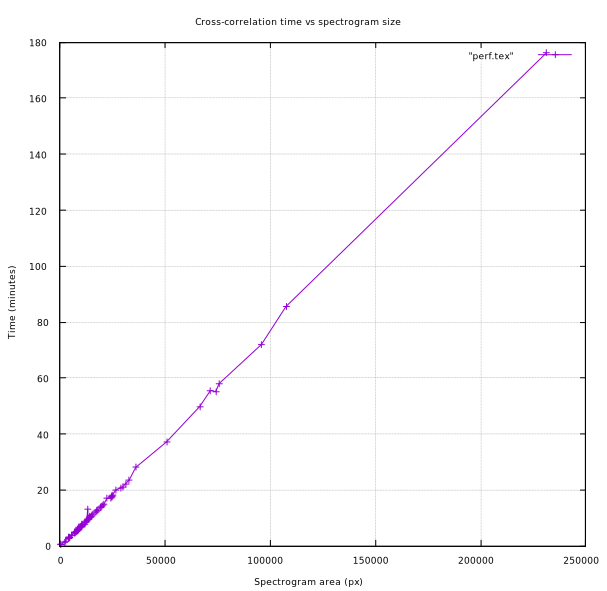
\includegraphics[width=1.0\textwidth]{ccm_time_sgram}
    \caption{}
  \end{subfigure}%
  \begin{subfigure}[b]{0.5\textwidth}
    \centering
    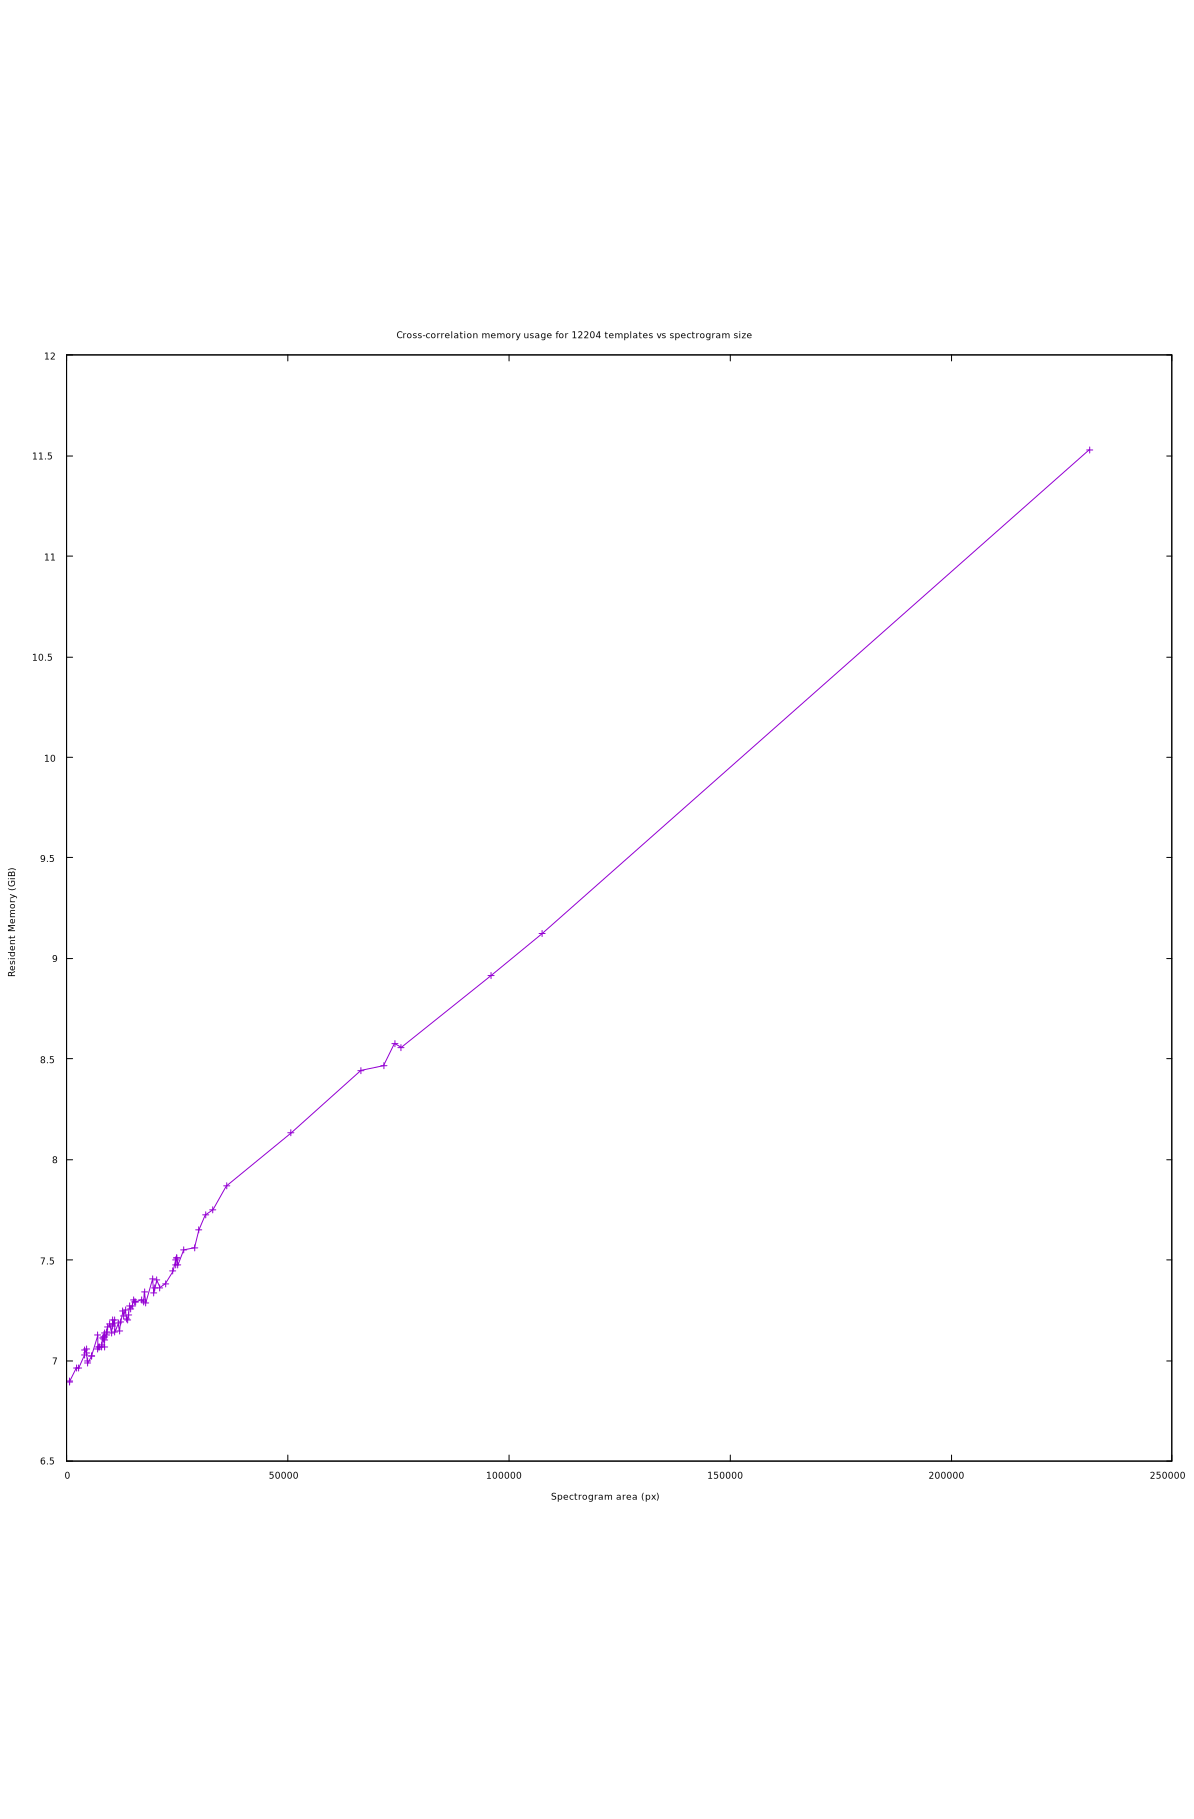
\includegraphics[width=1.0\textwidth]{ccm_mem_sgram}
    \caption{}
  \end{subfigure}
  \caption{Time (a) and resident memory (b) usages as pixel count increases for
  cross-correlation against 12204 templates}
\end{figure}

Further optimisations have been implemented.
In particular, dimensionality reduction is performed on templates and
spectrograms by blurring and reducing their size as seen in
Section~\ref{sec:extract}.

In addition, template matching is multithreaded using Python's |multiprocessing|
module.
Spectrograms are split into even chunks equalling the number of usable CPUs on
the machine, joining results upon completion.
This cuts the cost down to approximately $1/4$ of the original time.\\

Additional optimizations could, but have not been implemented:
\begin{itemize}[noitemsep]
  \item Template matching can be confined to the general area at which the template
    was extracted.
    This is possible if the frequency bands, or image coordinates at which a
    template was extracted is stored for this purpose.
    If implemented, the search area for template matching should be increased by some
    value to account for natural or artificial deviations.

  \item Open-CV's template matching function supports on-GPU calculations.
    Doing so would result in considerable gains in speed, however this requires
    an NVIDIA CUDA device (http://docs.opencv.org/2.4/modules/gpu/doc/introduction.html).

  \item Open-CV uses FFT.
    Fast Normalised Cross Correlation (FNCC) is a faster alternative to FFT based
    methods of template matching (TemplateMatchingusingFastNormalizedCrossCorrelationKaiBriechleandUweDHanebeck).
    Replacing calls to an implementation which uses FNCC would result in some 
    performance gains, however an existing implementation has not been found,
    and writing one from scratch is expensive without a guarantee of noticeable
    impact.
\end{itemize}

\subsection{Feature Vector Construction}
The template matching results are used to construct a feature vector for each
recording.
The feature vector of each sample therefore encodes the extent at which it's
recording contains similar characteristics to each species' song.
Feature vectors compose the training and test data for machine learning in
Chapter~\ref{cha:clf}.

The length of each feature vector is constant across all species and is equal to
the number of extracted templates.
The values of each element in the vector are derived from the template matching
results by taking the maximum value from the cross-correlation mapping.
The maxima intuitively gives us the highest matching probability for a template,
but discards information of other possible matches.
This extraction has shown promising results (\textcite{fodor2013}).


\chapter{CLASSIFICATION AND EVALUATION}

\section{Random Forests}

\section{Accuracy Evaluations}

\section{Classification}
With feature vectors constructed, we select a machine learning algorithm to
train and classify birdsong based on our model.
This section details the choice of algorithm, it's variations, performance and
tuning.

\subsection{Approaches to Classification}
obviously a classification task.
We are working with limited sample set, but high number of features.
The data is labelled, so we will select a supervised learning algorithm.
we must select a classifier which performs well with this data.
identifying the best classifier can be best done by cross validating each and
selecting the best performer.
For the purposes of testing our approach, a single algorithm was initially
chosen.

random forest is a good performer and is highly scalable (ref).
We chose this algorithm.

also might look at gradient boosted trees.

number of classifiers can be used
skim through some strengths and weaknesses

\subsection{Random Forest Classifier}
A random forest classifier is an ensamble of trees.
A node of a tree is split on an index of the feature vector.
Each Tree uses a new random sampling of the features.

we pick the random forest.
explain why we use this classifier
explain how it fits with the data we are working with

This is a multi-class classifier, returning the probabilities of each class
corresponding to the data given.
An alternative approach is possible, in which the classification of each species
is split into individual random forests, the final result of which is retrieved
by taking the maximum of all probabilities.
Using multiple binary classifiers allows other accuracy metrics to be used,
facilitating the accuracy evaluation of single species.

\subsection{Extremely Randomised Trees}
Extremely Randomised Trees is similar to a traditional Random Forest, however
however splitting is randomised, instead of being computed for optimal
performance.
This has the benefit of being faster, with the drawback of being more sensitive
to noisy features.\\

Using this classifier has seen no major accuracy or performance differences.
why do we use it, no reason??

\subsection{Parameter Selection}
show parameters available for RF
show initial parameters chosen and their performance
how did we pick these? (make something up)

Section~\ref{sec:tuning} explores semi-automatic parameter tuning and touches on
the issues of overfitting.

\section{Accuracy Evaluation}

a mention on differences in measuring accuracy for single-label vs multi
label classifier

mention any metrics that we do not use but are standard, and explain
why we do not use them.

\subsection{Validation Strategy}
10 times 10kfold

\subsection{Accuracy Metrics}
mean accuracy, f-score, etc
results

\subsection{AUC curve}
we dont use this but if we can construct one then show how we do and what
this tells us

\subsection{Confusion Matrix}
what it is, what it can show us
what it actually shows us

\section{Tuning}\label{sec:tuning}
In machine learning there is no single set of parameters or rule set which will
gaurantee optimal performance.
The only conclusive method to find optimal parameter values is to evaluate
the effects of changing them.
If done incorrectly however, tuning can lead to overfitting.

Overfitting can occur if tuning is performed on the entire dataset.
To reduce the chance of this, datasets should also be split into development
and evaluation sets.
Although we don't do this here, we do use 10-times 10-fold cross validation as
described in Section~\ref{sec:acc_eval}.
This mechanism coupled the good overfitting resistance exhibited by the random
forests algorithm should provide sufficiently valid results.

The parameter search algorithm and analysis of results are discussed in this
section.


\subsection{Gridsearch}
The most basic form of parameter search is exhaustive gridsearch.
A set of influential parameters are chosen, as well as a range of discrete
values to test.
Gridsearch then involves the exhaustive enumeration  of all possible parameter
value combinations.

We test each combination using the usual evaluation mechanism with the following
search space:
\begin{itemize}
  \item Estimators: 10, 500, 5000, 10000
  \item Max features: Sqrt, log2, num features
  \item min samples split: 2, 10, 100
  \item min samples leaf: 1 10 100
  \item max depth: None, 5, 10, 100, 200
\end{itemize}

The effect of each parameter is described in Section~\ref{sec:param}.

..we can use oob to help eval but it's reportedly not as certain as splitting
train/test

we do this multithread

NOTE NOTE NOTE
variance uncertainty with low number of samples

%0 doing params: 0/8 {'max_features': 'sqrt', 'min_samples_split': 2, 'n_estimators': 10, 'max_depth': None, 'min_samples_leaf': 1}
%/usr/lib/python2.7/site-packages/sklearn/metrics/classification.py:1113: UndefinedMetricWarning: Precision and F-score are ill-defined and being set to 0.0 in labels with no predicted samples.
%  'precision', 'predicted', average, warn_for)
%0 params: 0/8 {'max_features': 'sqrt', 'min_samples_split': 2, 'n_estimators': 10, 'max_depth': None, 'min_samples_leaf': 1}
%accuracies: 0.792083333333 std. 0.0846756474896
%fscores: 0.774496031746 std. 0.0912070497428
%precisions: 0.807 std. 0.0956255638247
%recalls: 0.792083333333 std. 0.0846756474896
%
%0 doing params: 1/8 {'max_features': 'sqrt', 'min_samples_split': 2, 'n_estimators': 500, 'max_depth': None, 'min_samples_leaf': 1}
%0 params: 1/8 {'max_features': 'sqrt', 'min_samples_split': 2, 'n_estimators': 500, 'max_depth': None, 'min_samples_leaf': 1}
%accuracies: 0.828958333333 std. 0.0882308269226
%fscores: 0.815523809524 std. 0.0966295635391
%precisions: 0.848388888889 std. 0.0972153211836
%recalls: 0.828958333333 std. 0.0882308269226
%
%0 doing params: 2/8 {'max_features': 'sqrt', 'min_samples_split': 2, 'n_estimators': 5000, 'max_depth': None, 'min_samples_leaf': 1}
%0 params: 2/8 {'max_features': 'sqrt', 'min_samples_split': 2, 'n_estimators': 5000, 'max_depth': None, 'min_samples_leaf': 1}
%accuracies: 0.8425 std. 0.0817020898232
%fscores: 0.83025 std. 0.0894293997584
%precisions: 0.864009259259 std. 0.0897250797427
%recalls: 0.8425 std. 0.0817020898232
%
%0 doing params: 3/8 {'max_features': 'sqrt', 'min_samples_split': 2, 'n_estimators': 10000, 'max_depth': None, 'min_samples_leaf': 1}
%0 params: 3/8 {'max_features': 'sqrt', 'min_samples_split': 2, 'n_estimators': 10000, 'max_depth': None, 'min_samples_leaf': 1}
%accuracies: 0.847708333333 std. 0.0785720542453
%fscores: 0.835843253968 std. 0.0857529898424
%precisions: 0.86990625 std. 0.0854490334312
%recalls: 0.847708333333 std. 0.0785720542453
%
%0 doing params: 4/8 {'max_features': 'log2', 'min_samples_split': 2, 'n_estimators': 10, 'max_depth': None, 'min_samples_leaf': 1}
%0 params: 4/8 {'max_features': 'log2', 'min_samples_split': 2, 'n_estimators': 10, 'max_depth': None, 'min_samples_leaf': 1}
%accuracies: 0.8225 std. 0.0965048933705
%fscores: 0.80795 std. 0.106203027383
%precisions: 0.841780555556 std. 0.109063062903
%recalls: 0.8225 std. 0.0965048933705
%
%0 doing params: 5/8 {'max_features': 'log2', 'min_samples_split': 2, 'n_estimators': 500, 'max_depth': None, 'min_samples_leaf': 1}
%0 params: 5/8 {'max_features': 'log2', 'min_samples_split': 2, 'n_estimators': 500, 'max_depth': None, 'min_samples_leaf': 1}
%accuracies: 0.824236111111 std. 0.0939180335682
%fscores: 0.80928968254 std. 0.10361060088
%precisions: 0.842261574074 std. 0.106871892753
%recalls: 0.824236111111 std. 0.0939180335682
%
%0 doing params: 6/8 {'max_features': 'log2', 'min_samples_split': 2, 'n_estimators': 5000, 'max_depth': None, 'min_samples_leaf': 1}
%0 params: 6/8 {'max_features': 'log2', 'min_samples_split': 2, 'n_estimators': 5000, 'max_depth': None, 'min_samples_leaf': 1}
%accuracies: 0.825297619048 std. 0.0924877228783
%fscores: 0.810106575964 std. 0.102024617976
%precisions: 0.842986111111 std. 0.105094010389
%recalls: 0.825297619048 std. 0.0924877228783
%
%0 doing params: 7/8 {'max_features': 'log2', 'min_samples_split': 2, 'n_estimators': 10000, 'max_depth': None, 'min_samples_leaf': 1}
%0 params: 7/8 {'max_features': 'log2', 'min_samples_split': 2, 'n_estimators': 10000, 'max_depth': None, 'min_samples_leaf': 1}
%accuracies: 0.826302083333 std. 0.090884670484
%fscores: 0.811121031746 std. 0.100457879026
%precisions: 0.844520833333 std. 0.10332019009
%recalls: 0.826302083333 std. 0.090884670484



\subsection{validation curves}
we tune based on best performing params in gsearch
possibly biased towards validation dataset
for better generalization estimation compute score on different set
(already mentioned above)

we can use this to check over/under fitting?
check influence of single parameter on training and validation scores
if both are low, clf is undefitting
if training is high, valid is low, clf is overfitting
low training, high validation not possible usually

coarse-to-fine search gridsearch, if we have the time

\subsection{Learning Rate}
learning curve
shows validation/training score for varying train sample count.
shows how clf may benefit from additional samples if at all
shows if clf suffers from variance or bias error
if validation and training score converge to a low value with more training samples,
we don't benefit. might have to change parameters or choose different clf which
has lower bias

if training score is higher than valid score, we benefit from adding training
samples probably, increasing generalisation

is this useful for RF?

\section{Feature Importance}
Without reduction, feature counts per species range from 2000 to 3000.
Each new sample to be classified will involve template matching against all
templates of all species.
For the n selected this means n cross correlations, which takes approximately
n time.
Feature reduction is therefore an important aspect for performance improvement.
It is also helpful in determining what kind of features are most helpful, which
may be used to help eliminate features early on before they are used in any
heavy computation.

\subsection{Measuring Feature Importance}
One method for measuring the impact of each feature is through the mean decrease
in accuracy.
With this method, the impact of removing each feature one-by-one is measured.
This method may be sensitive to the random nature of the classifier, so multiple
runs may be required to eliminate any variance (is this true?).
This can be prohibitively expensive.

\subsubsection{Feature importance in random forests}
Because the nodes of trees in a random forest correlate directly with a specific
feature, it is possible to directly measure or estimate the importance of each
feature by determining the probability of a node in a tree being traversed over 
the number of nodes in the forest.
This is known as the mean decrease impurity, or gini impurity, and it can be
measured directly after a forest has been trained, or estimated beforehand \bfseries{(is this true?)}.

This project makes use of the .... measure.

\subsection{Results}
Measuring feature importances exposes x of y features to be completely useless
for specifying or discriminating classes of species.
Removing these features results in no change in accuracy.
Performance increases are observed in both feature extraction
\bfseries{(is it still extraction? build feature vector)} and classification.
The greatest increase in performance was observed in the template matching stage
with a mean decrease of x minutes.

\bfseries{graph of feature importances}

\bfseries{to do:}
Further reductions were made to the feature set in effort to reduce the feature
count as much as possible while retaining a consistent accuracy.
etc etc was found.
lots of graphs



\chapter{CONCLUSIONS}

%- a summary and critical evaluation of what has been achieved
%
%- some feedback on what you personally have learned from the project
%
%- some thoughts to what you would do with more time (what are the
%  most important tasks not carried out?), and also how you would
%  change your approach if you were tarting over, based on what you
%  know now.

\section{Summary}
This report describes the solution developed for the task of automatic birdsong
recognition.
Existing approaches to relevant problems were used as a starting point.
The approach reduces the initial problem to image recognition using spectrograms
of the 2211 field recordings sourced from Xeno-canto.
Image processing techniques were investigated to maximise template quality.
A random forest classifier was selected to classify 240 of the samples using the
cross-correlation results.
After tuning, the model was evaluated using 10-times 10-fold cross validation, 
achieving a peak accuracy of 88\%, and F1 score of 87\%.
Finally, feature importances were analysed to rank templates and perform further
feature reductions to improve scalability.

\section{Reflection}
An open-ended project such as this has scope for exploratory research.
Regardless of the approach taken, the nature of the project touches on many
facets of computer science.
Our approach focuses on computer vision and machine learning, touching on
performance computing with (relatively) large amounts of data.\\

Although good results were achieved, these could have been improved.
Model performance is highly dependent on the features used, and this area
lacks in sophistication and validation.
Although we learned about a few computer vision techniques for this, we could
have increased the breadth and depth of our investigations in this area.

We are confident that the choice of classifier was a good one.
A lot was learned about machine learning methodologies, although there exists
a lot of contradictory findings and advice, it is the general consensus that
with whatever application, it is the data that shapes the approach and the only
conclusive evaluation to be made is directly based on this.

Given more time, other classifiers could be evaluated as well,
however validation was limited immensely by the lack of data processed data.
A total of 20 samples per label was not enough to confidently measure the
performance of the classifier.
Given more data, a further separation of development and validation could have
been done, leading to a more representative evaluation.\\

The lack of data stems from the immense processing power required to
cross-correlate all 35773 templates.
This makes it extremely expensive to evaluate new template extractions.
With this in mind it would have been justifiable to seek external computing
resources early on, and to spend more time on optimisations.
With this in mind, Python was not the right choice in terms of performance.\\


On the topic of software engineering, recommended practices were not observed.
The exploratory nature of the project has lead to many quick iterations and hacks
in the software.
Some effort was expended to restructure large portions of the code to make it
more robust to future changes, however this quickly deteriorated.
This was due to the fact that no strict requirements were produced for the
program's functionality.
It was always inteded as a test-bed for the explored methods, and so there exists
a tradeoff between developing the framework and developing the solution.
We have learned instead that simplicity is key: equal performance would have
been achieved by splitting the program into discrete artefacts, and transferring
data through files instead of in-memory.


\section{Future Work}


%You currently do not at all address standard SE issues in terms of the
%design, implementation and testing of the software you produced. This
%is fine with me because I am much more interested in what you have
%written about. I still felt I should point this out in case you want
%to squeeze in a summary.
%For this I plan to include some diagrams to describe the flow of data and
%how the software is structured.
%I am yet to write about my development process, but it will not be
%anything too in depth.
%I also intend to discuss any difficulties or matters of interest
%retrospectively in the conclusion.
%Some SE matters are briefly discussed in some of the texts, but I did not
%want to dive into too much detail since implementation details are not the
%main concern.
%No strict testing took place. Something to reflect on again.



\printbibliography

\begin{appendices}
  \section{Sample and Template counts per Species}\label{app:samples}

%\begin{table}[!htb]
  %\centering
  \begin{longtable}{l r r}
Species                         &Spectrograms &Templates \\ \hline
Common Blackbird                &101  &38818 \\
Eurasian Blackcap               &99   &42274 \\
Eurasian Wren                   &94   &17431 \\
Common Chiffchaff               &66   &10273 \\
Grey-breasted Wood Wren         &66   &5603  \\
Spotted Towhee                  &53   &3583  \\
Garden Warbler                  &48   &18258 \\
Eurasian Blue Tit               &44   &4228  \\
Common Whitethroat              &42   &9858  \\
Great Reed Warbler              &40   &12762 \\
Rufous-browed Peppershrike      &39   &3491  \\
River Warbler                   &38   &11291 \\
Yellowhammer                    &38   &6442  \\
White-breasted Wood Wren        &38   &4123  \\
Eurasian Reed Warbler           &37   &30421 \\
Common Grasshopper Warbler      &36   &3035  \\
Corn Bunting                    &32   &3177  \\
Common Reed Bunting             &31   &2850  \\
Northern Mockingbird            &29   &8333  \\
Common Cuckoo                   &29   &4854  \\
Common Redstart                 &27   &10774 \\
Common Rosefinch                &27   &3733  \\
Ortolan Bunting                 &24   &2686  \\
Chestnut-breasted Wren          &24   &2524  \\
Western Meadowlark              &23   &8256  \\
Pale-breasted Spinetail         &22   &2717  \\
White-throated Toucan           &21   &6814  \\
European Greenfinch             &21   &2844  \\
Pin-striped Tit-Babbler         &20   &2575  \\
Ferruginous Pygmy Owl           &18   &5000  \\
American Robin                  &18   &3515  \\
Barred Antshrike                &16   &2478  \\
Black-striped Sparrow           &15   &2510  \\
Lesser Shortwing                &15   &1656  \\
Green-winged Saltator           &15   &1644  \\
Black-faced Antbird             &15   &1514  \\
Pale-breasted Thrush            &14   &2955  \\
Plain-tailed Wren               &14   &2847  \\
Channel-billed Toucan           &14   &1619  \\
Plumbeous Vireo                 &14   &1094  \\
Common Potoo                    &13   &3690  \\
Grace's Warbler                 &13   &2069  \\
Swainson's Thrush               &13   &2044  \\
Rufous-capped Warbler           &13   &1692  \\
Greenish Warbler                &13   &1668  \\
White-breasted Tapaculo         &13   &1525  \\
Tawny Owl                       &13   &1133  \\
Loggerhead Shrike               &12   &3281  \\
Undulated Tinamou               &11   &4184  \\
Collared Owlet                  &11   &3642  \\
Great-tailed Grackle            &11   &2424  \\
Japanese Bush Warbler           &11   &1628  \\
Giant Antshrike                 &11   &605   \\
Rattling Cisticola              &10   &0     \\
Bell's Vireo                    &10   &0     \\
White-throated Sparrow          &10   &0     \\
Scrub Greenlet                  &10   &0     \\
Olive Warbler                   &10   &0     \\
Laughing Falcon                 &10   &0     \\
Red-winged Blackbird            &9    &0     \\
Common Hawk-Cuckoo              &9    &0     \\
Yellow-browed Sparrow           &9    &0     \\
Eastern Meadowlark              &9    &0     \\
Slaty-breasted Wood Rail        &9    &0     \\
Sumichrast's Wren               &9    &0     \\
Plain-crowned Spinetail         &9    &0     \\
Yellow-eyed Junco               &9    &0     \\
Spotted Nightingale-Thrush      &9    &0     \\
Japanese White-eye              &9    &0     \\
Painted Bunting                 &8    &0     \\
Southern Yellowthroat           &8    &0     \\
Great Tinamou                   &8    &0     \\
Sooty Antbird                   &8    &0     \\
Styan's Grasshopper Warbler     &8    &0     \\
Yellow-throated Vireo           &7    &0     \\
Connecticut Warbler             &7    &0     \\
Hooded Siskin                   &7    &0     \\
Fire-tufted Barbet              &7    &0     \\
Duida Woodcreeper               &7    &0     \\
Gartered Trogon                 &7    &0     \\
Eurasian Treecreeper            &7    &0     \\
Buff-browed Foliage-gleaner     &7    &0     \\
Eurasian Golden Oriole          &7    &0     \\
White-bellied Antpitta          &7    &0     \\
Grey Antwren                    &7    &0     \\
Southern Boubou                 &7    &0     \\
Western Orphean Warbler         &6    &55    \\
Bay Wren                        &6    &10    \\
Recurve-billed Bushbird         &6    &0     \\
Golden-crowned Sparrow          &6    &0     \\
Splendid Sunbird                &6    &0     \\
Moustached Wren                 &6    &0     \\
Collared Antshrike              &6    &0     \\
Violaceous Euphonia             &6    &0     \\
Siberian Blue Robin             &6    &0     \\
Henna-hooded Foliage-gleaner    &6    &0     \\
Baillon's Crake                 &6    &0     \\
Paradise Jacamar                &6    &0     \\
Rufous-vented Tapaculo          &6    &0     \\
Ashy-headed Greenlet            &6    &0     \\
Spotless Starling               &6    &0     \\
Eastern Woodhaunter             &6    &0     \\
White-throated Screech Owl      &6    &0     \\
Lineated Foliage-gleaner        &6    &0     \\
Orange-breasted Bushshrike      &5    &10    \\
Yellow Grosbeak                 &5    &0     \\
Tanager Finch                   &5    &0     \\
Foothill Schiffornis            &5    &0     \\
Singing Quail                   &5    &0     \\
Esmeraldas Antbird              &5    &0     \\
Spectacled Owl                  &5    &0     \\
Dark-capped Bulbul              &5    &0     \\
Marico Sunbird                  &5    &0     \\
Yellow-bellied Elaenia          &5    &0     \\
Buff-cheeked Greenlet           &5    &0     \\
Audubon's Oriole                &5    &0     \\
Curve-billed Scythebill         &5    &0     \\
Wedge-billed Woodcreeper        &4    &341   \\
California Quail                &4    &126   \\
White-throated Toucanet         &4    &0     \\
Red-fan Parrot                  &4    &0     \\
Black-cowled Saltator           &4    &0     \\
Western Wood Pewee              &4    &0     \\
Variegated Antpitta             &4    &0     \\
Zigzag Heron                    &4    &0     \\
Fan-tailed Cuckoo               &4    &0     \\
Greater Thornbird               &4    &0     \\
Blue-chested Hummingbird        &4    &0     \\
Green-backed Sparrow            &4    &0     \\
Varied Bunting                  &4    &0     \\
Ferruginous Partridge           &4    &0     \\
White-vented Violetear          &4    &0     \\
Golden-rumped Euphonia          &3    &379   \\
White-fronted Honeyeater        &3    &336   \\
White-necked Puffbird           &3    &82    \\
White-spectacled Warbler        &3    &53    \\
White-shouldered Antbird        &3    &0     \\
Rufous-tailed Hummingbird       &3    &0     \\
Blue-winged Pitta               &3    &0     \\
Jerdon's Leafbird               &3    &0     \\
Olive Thrush                    &3    &0     \\
Azure Jay                       &3    &0     \\
Johannes's Tody-Tyrant          &3    &0     \\
Short-billed Leaftosser         &3    &0     \\
Japanese Quail                  &3    &0     \\
Chestnut-bellied Thrush         &3    &0     \\
Crested Lark                    &3    &0     \\
Emerald Toucanet                &3    &0     \\
Greater Hoopoe-Lark             &3    &0     \\
Chestnut-bellied Nuthatch       &3    &0     \\
Forest Elaenia                  &3    &0     \\
Long-billed Pipit               &3    &0     \\
Moustached Puffbird             &3    &0     \\
Choco Tapaculo                  &3    &0     \\
Wedge-tailed Grass Finch        &3    &0     \\
Pearly Antshrike                &2    &173   \\
Little Cuckoo-Dove              &2    &139   \\
Bahama Oriole                   &2    &109   \\
White-eared Brown Dove          &2    &97    \\
Plush-crested Jay               &2    &96    \\
Grey-throated Warbler           &2    &92    \\
White-naped Jay                 &2    &56    \\
Pririt Batis                    &2    &35    \\
Black-goggled Tanager           &2    &33    \\
Scarlet-rumped Trogon           &2    &5     \\
Arafura Fantail                 &2    &0     \\
Yellow-crowned Elaenia          &2    &0     \\
Bronzy Jacamar                  &2    &0     \\
Philippine Coucal               &2    &0     \\
Flammulated Bamboo Tyrant       &2    &0     \\
Russet Nightingale-Thrush       &2    &0     \\
Hepatic Tanager                 &2    &0     \\
Solitary Tinamou                &2    &0     \\
Jerdon's Nightjar               &2    &0     \\
Cuban Vireo                     &2    &0     \\
Streak-breasted Treehunter      &1    &1118  \\
Emei Shan Liocichla             &1    &350   \\
Crimson-backed Tanager          &1    &261   \\
Curve-winged Sabrewing          &1    &236   \\
Eastern Nicator                 &1    &169   \\
Yellow-breasted Boatbill        &1    &160   \\
Tiny Tyrant-Manakin             &1    &149   \\
Mountain Wren-Babbler           &1    &119   \\
Winifred's Warbler              &1    &116   \\
Negros Scops Owl                &1    &109   \\
Green-chinned Euphonia          &1    &98    \\
Sombre Rock Chat                &1    &83    \\
Cherrie's Antwren               &1    &39    \\
Sand Martin                     &1    &17    \\
Yellow-breasted Pipit           &1    &13    
  \end{longtable}
%\end{table}

\end{appendices}

\end{document}
